\subsubsection*{I.8.18}
а)
\begin{figure}[h]
	\center{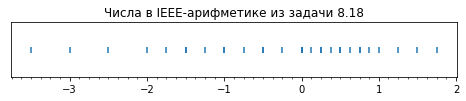
\includegraphics{parts/img/I_8_18.png}}
\end{figure}\\
В данной модели удалось представить 23 числа.\\
б) 
$$\varepsilon_{маш} = 0,25$$
забавная ситуация, что слева от единицы следующее число располагается на расстоянии $0,125$, а справа --- $0,25$. На всякий случай взял $0,25$, так как в методичке было равенство $1 + \varepsilon_{маш}$.
$$\text{OFL} = 1,75$$
$$\text{UFL} = 0,125$$